\myChapter{State of the Art on Anomaly Detection in DNS Transactions}{}\label{chapEditionStructure}
%\myMinitoc{Profondeur de la minitoc (section|subsection|subsubsection)}{Titre de la minitoc}
\myMiniToc{}{Contents}

%\mySectionStar{Titre}{Titre court}{Ajouter à la table des matières? (false|true|chapter|section|subsection|subsubsection -section par défaut-)}
\mySection{Introduction}{}
Anomaly detection in DNS transactions is crucial for identifying malicious activities, such as botnet command and control, DDoS attacks, and data exfiltration. This overview will cover traditional rule-based and statistical methods, as well as modern machine learning techniques, including supervised and unsupervised learning approaches.
\mySection{Traditional Anomaly Detection Techniques}{}
Traditional detection-based techniques in DNS anomalies focus on identifying deviations from normal DNS behavior to detect malicious activities or irregularities. These techniques generally fall into several categories:
\subsection{signature-based system}
Signature-based detection involves using pre-defined patterns or signatures of known malicious DNS queries or responses. This method is effective against known threats but struggles with new or unknown threats. In this context,Smith et al \cite{smith2019evaluation} proposed an evaluation of signature-based anomaly detection in DNS traffic and obtained 85\% detection rate and a false positive rate of 10\%. however, their appraoch was limited in their inability to detect new threats since they rely on predefined patterns. Next,Lee et al \cite{lee2020novel} proposed a novel rule-based anomaly detection system  tailored to DNS traffic characteristics.The proposed system employs a rule-based approach, where specific rules are formulated based on known patterns of normal DNS behavior. These rules are designed to flag deviations from expected DNS traffic patterns, indicating potential anomalies. The system utilizes features such as query types, query frequency, and domain reputation to establish and identify deviations. They had 88\% detection rate and 12\% false positive rate but however, their method was limited in that they required constant updating of rules or signatures. Next?,Kumar et al \cite{kumar2021dns} futher proposed set of predefined rules to identify anomalies.They obtained 83\% detection rate and 14\% false positive rate. Their model was Prone to false positives and lacks adaptability  and scalability for increasing as the volume of DNS traffic increases.



\subsection{statistical methods}
The statistical approach to DNS traffic analysis for anomaly detection is a sophisticated method aimed at identifying irregularities or deviations from normal behavior within DNS data flows. This approach relies on statistical techniques to establish baseline patterns of DNS activity and subsequently detect anomalies that may indicate malicious or suspicious activities. Here's an overview of the key statistical techniques employed in this approach:\\
\textbf{Baseline Establishment:}
Before detecting anomalies, it's crucial to establish a baseline of normal DNS traffic behavior. This involves analyzing historical DNS data to understand typical patterns in query volumes, types of queries, response times, and other relevant metrics. Statistical methods such as mean, median, mode, and standard deviation are utilized to quantify these patterns and create a reference point for normalcy.\\
\textbf{Z-Score Analysis:}
Z-score analysis is a common statistical technique used to identify outliers or anomalies in a dataset. In the context of DNS traffic analysis, z-scores are calculated for various metrics such as query frequency, response times, or query types. A z-score measures how many standard deviations a data point is from the mean of the dataset. Data points with z-scores beyond a predefined threshold are flagged as anomalies, indicating potentially suspicious DNS activity\\
\textbf{Time Series Analysis:}
Time series analysis is another essential statistical method used in DNS traffic analysis. It involves studying patterns and trends in DNS data over time to detect anomalies. By applying techniques such as moving averages, exponential smoothing, or autoregressive integrated moving average (ARIMA) modeling, analysts can identify irregularities in DNS traffic patterns that may signify malicious activities or unusual network behavior. Following this approach, Wang et al \cite{wang2021statistical} proposed a methodology for establishing baseline behavior patterns using historical DNS data and described how statistical measures such as z-score analysis, time series analysis could applied to detect deviations from the baseline indicative of suspicious activities. They obtained 87\% detection rate and 15\% false positive rate. But were computationally intensive since they were not scalable,dificulties in features extraction. Again, Chen et al \cite{chen2022comparative} proposed a model using clustering algorithms  notably k-means and established a correlation analysis among features, and obtained an overall performance of 85\% detection rate, and a 16\% false positive rate which was as a result of lack of scalability in their model, the choice of the number of clusters also affected this results. \cite{rodriguez2022time} worked on the same dataset but used a different approach, instead of using clustering algorithms and correlation analysis, they proposed and exponentially Weighted Moving Average method for smoothing time series data to highlight trends and anomalies, DBSCAN (Density-Based Spatial Clustering of Applications with Noise Used to find core samples of high density and expand clusters from them rather than limiting the number of clusters at the begining as others did. Their peformance was good as compared to that of \cite{chen2022comparative},that is,89\% detection rate and 14\% false positive rate. But this method was also limited since it required extensive historical data and not scalable. Pavel Čeleda et Radek Kreje. \cite{eunice2014} Proposed a monitoring DNS traffic using both standard and extended flow records focusing on port-based identification traffic based on the assigned TCP and UDP port number 53,flow aggregation of packets with common properties into flows until termination, and extending these records with DNS-specific information. Their model had a significant performance and a low positive rate but however also had some limits on the flow record size and detection complexity. Kim et al. \cite{kim2023improving} Proposed an improved statistical model based on extended flow records to include DNS-specific information, such as queried domain names and types, response codes, and response data to allows for more detailed analysis of DNS traffic without significantly increasing the flow record size and also optimized flow cache to handle high volume of DNS traffic. An accuracy of 91\% detection rate and 11\% false positive rate was obtained which improved the previous models but was limited because of the high complexity since the flow rate was extended.



\mySection{Machine Learning-Based Techniques in binary and multiple classification}{}
Machine learning involves training algorithms on data to identify patterns and make predictions.In DNS traffic detection, ML can help identify malicious traffic by learning from historical data.

\textbf{Binary vs. Multi-Class Classification}\\
\textbf{Binary Classification:} Here, the aim is to  differentiates between two classes, such as benign(non malicious traffic) and malicious traffic.
Binary classification is a core task in machine learning where data is divided into two distinct categories. It finds extensive applications in domains like spam detection, medical diagnosis, and fraud detection. Several algorithms like logistic regression, support vector machines, decision trees, and neural networks are commonly used for binary classification tasks.
Evaluation of binary classifiers involves metrics such as accuracy, precision, recall, F1 score, and AUC-ROC, providing insights into model performance. In DNS anomaly detection, binary classification aims to classify DNS queries as normal or anomalous, leveraging features like query type, response time, and query frequency.
Challenges include dealing with class imbalance, selecting relevant features, avoiding overfitting, and ensuring real-time processing capabilities. Despite these challenges, binary classification serves as a robust framework for effective anomaly detection across various domains.Gupta et al.\cite{bilge2011exposure} Proposed a random forest approach for DNS anomaly detection on trained on labeled data. Their datasets was made up of bengns and attacks where at the end of thier training, the obtained a detection rate of 91\% and a 9\% false positive rate,but how ever had some limits in their model resulted in overfitting on small datasets. Next,Patel et al \cite{patel2022dns} Proposed an approach using support vector machines model to adress this problem and obtained a detection rate of 89\% and a 10\% false positive rate which was not encouraging since their model was sensitive to parameter selection.
\begin{comment}
\textbf{Multi-Class Classification: }
In multiclass classification, there are more than two possible outcomes or categories that the input instances can be classified into. These classes can be mutually exclusive  or non-mutually exclusive. For example the classification of DNS traffics into benigns, attacks or suspicious (which needs to be further analize). Based on this approach, researchers have carried out some researches on this and some of which are describe as follows: Johnson et al. \cite{johnson2023unsupervised} Proposed an Unsupervised DNS Anomaly Detection with Self-Organizing Maps (SOMs) trained a SOM on DNS traffic data and obtained a 90\% detection rate and a 10\% false positive rate and was limited since they required high computational resources and complexity, not scalable. \cite{Kai2019Anomaly}. Proposed an approach  to
detect general DNS anomalies that are statistically different from normal behavior using Big Data, given that DNS are often used as a covert channel for attackers to perform malicious activities e.g. data exfiltration. It was beneficial and proved to be crucial in any enterprise network since they used  GMM with two clusters, their
detection model was able to detect data exfiltration anomaliescwith a 95\% detection rate. Further to that,they used SOM for cluster analysis to determine if there are any visible clusters in the NetFlow dataset. However, given the nature of their network traffic collected from multi enterprise network of different organizations, no fixed number of clusters could be obtained due to the diversity of network traffic and the
varying traffic behavior of how different organizations operates, their estimation techniques using BIC/AIC
has been selected to determine the optimal number of
components/clusters for the GMM model. However, limited to
only data exfiltration anomalies, that is not able to detect other kinds of DNS anomalies other than
data exfiltration.

\textbf{Their model}

\begin{figure}[ht!]
    \centering
    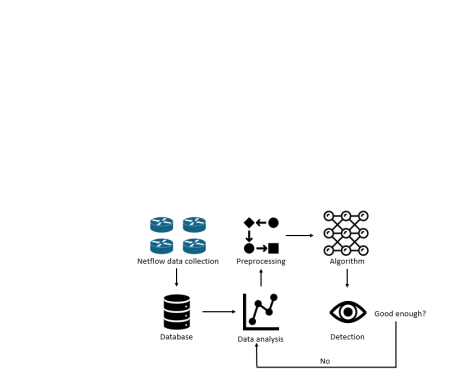
\includegraphics[width=1\linewidth]{netflow.png}
    \caption{architecture of Vivek Balachandran,Kelvin Soh Boon Kai\cite{Kai2019Anomaly}}
    \label{fig:enter-label}
\end{figure}
\end{comment}


\mySection{Supervised machine learning solution of binary classification of   ;;;;}{}
\mySection{supervised learning solution of multiple classification of bakro et al.}{} This study proposes a hybrid feature selection approach using the grasshopper optimization algorithm (GOA) and the genetic algorithm (GA) to enhance IDS performance by efficiently selecting optimal features. A random forest (RF) classifier, trained on these features, benefits from addressing data imbalance with ADASYN for minority class oversampling and random under-sampling (RUS) for the majority class \cite{cloud_ids2021}. Evaluated on three datasets (UNSW-NB15, CIC-DDoS2019, and CIC Bell DNS EXF 2021), the approach achieved accuracies of 98\%, 99\%, and 92\%, respectively. The hybrid IDS outperformed other classifiers and state-of-the-art methods, consistently delivering superior multi-class classification performance.
Based on the CIC Bell DNS EXF 2021 and the results of 92\% obtined, we noticed the limitations Our goal is to improve the performance of neural network classifiers by adjusting various parameters, including the n, connection density, selection of activation functions, and the number of training epochs. Additionally, we intend to implement systematic hyperparameter tuning for the classifiers using methods such as grid search, random search, and metaheuristic algorithms.
\subsection{performance metrics}
\mySection{Conclusion}{}